\documentclass{beamer}
\begin{document}
\title{Hierarchical Path-Finding}
\author{Addie Audette, Bug Lee, Annorah Lewis, Luke Marks}
\date{December 12, 2022} 

\frame{\titlepage} 

\frame{\frametitle{Table of contents}\tableofcontents} 


\section{Path finding background} 
\frame{\frametitle{Path finding} 
You are given
\begin{itemize}
  \item Starting location $S$
  \item Destination location $D$
\end{itemize}

\begin{figure} 
\centering
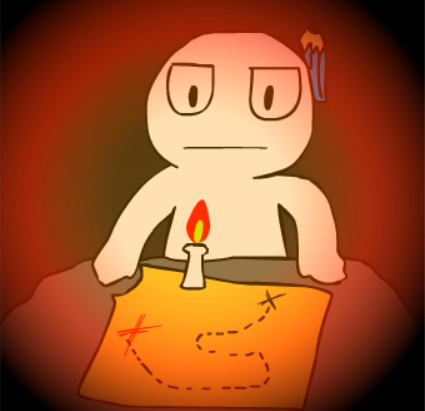
\includegraphics[scale=0.5]{imgs/path_finding.png}
\end{figure}
}

\frame{\frametitle{Path finding} 
You want to avoid path from $S$ to $D$ that are 
\begin{itemize}
  \item Impossible
  \item Dangerous
  \item Unnecessary
\end{itemize}

\begin{figure} 
\centering
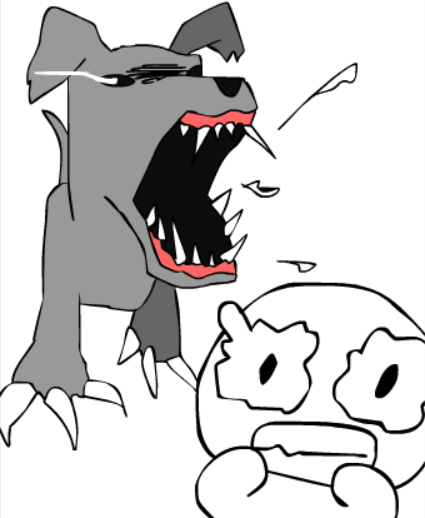
\includegraphics[scale=0.4]{imgs/dangerous_path.png}
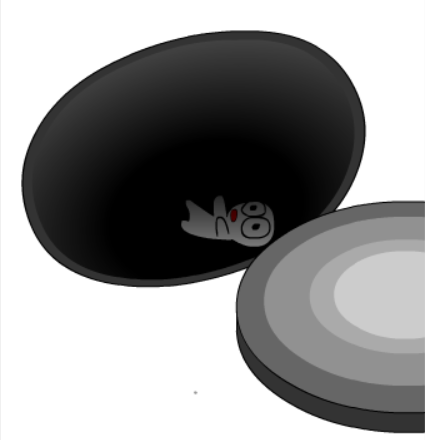
\includegraphics[scale=0.4]{imgs/wrong_path.png}
\end{figure}
}

\subsection{Grid graph}
\frame{\frametitle{Viewing world with grid graph} 
Imagine world is made of grid, like Mindcraft...

\begin{figure} 
\centering
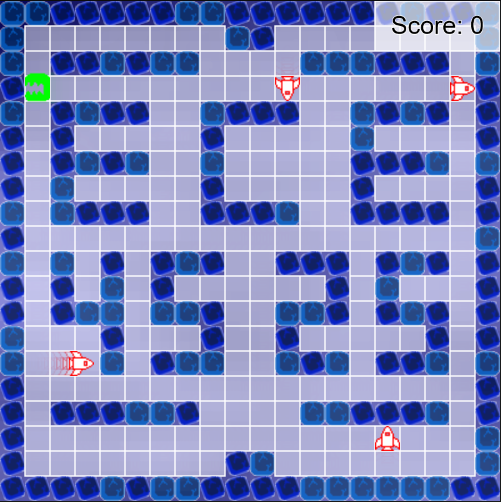
\includegraphics[scale=0.4]{imgs/grid_world.png}
\end{figure}
}

\frame{\frametitle{Viewing world with grid graph} 
\begin{itemize}
  \item Each cell is a vertex and has an edge to adjacent cells.
  \item No edges between cells and walls/obstacles
  \item So, each vertex can have up to degree 4 and edges are undirected with weight 1.
\end{itemize}

\begin{figure} 
\centering
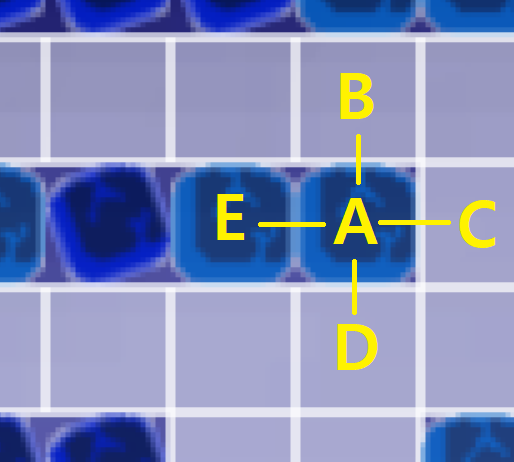
\includegraphics[scale=0.4]{imgs/adjacency.png}
\end{figure}
}

\frame{\frametitle{Back to path finding} 
Now, using the grid graph, how can we find the shortest path from $S$ to $D$?
\begin{figure} 
\centering
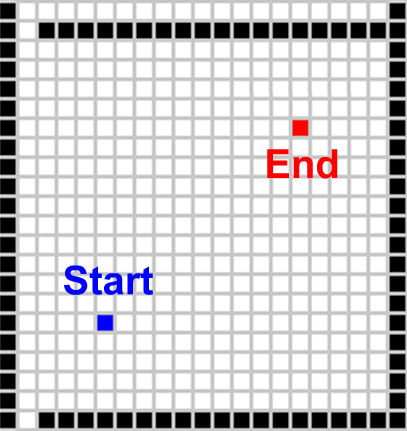
\includegraphics[scale=0.4]{imgs/start_and_end.png}
\end{figure}
}

\section{Shortest path algorithms}
\subsection{Dijkstra}
\frame{\frametitle{Dijkstra}
\begin{itemize}
  \item Dijkstra algorithm finds the shortest path to all the vertices from source $s$, given that the graph $G = (V, E)$ contains only non-negative weight for all edges\cite{CLRS}. 
  \item In other words, it forms the tree that represents the shortest paths to all of the vertices in the graph. 
\end{itemize}

\begin{figure} 
\centering
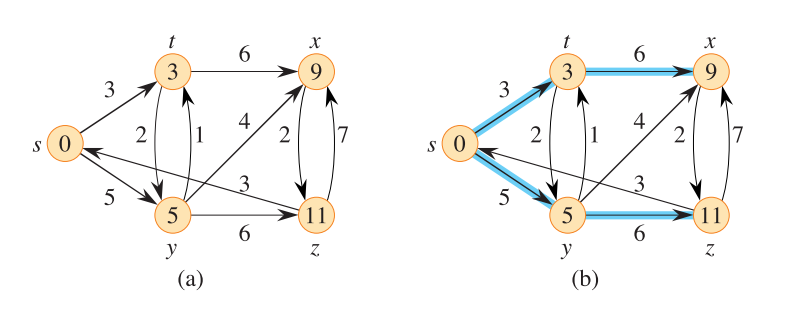
\includegraphics[scale=0.5]{imgs/shortest_path_tree.png}
\caption{(a) A weighted, directed graph with source $s$. (b) The blue edges represent the shortest-path tree rooted at the source $s$. The figure was taken from \textit{Introduction to Algorithms} by CLRS\cite{CLRS}.} 
\end{figure}
}

\frame{\frametitle{Dijkstra Algorithm}
Dijkstra algorithm is a type of greedy algorithm where it makes a locally optimal decision in each step. The following describe the high-level idea:

\begin{enumerate}
    \item At first, the source vertex only knows the distance to its neighbors and treats other vertices as if they are infinitely far away. 
    \item Among the univisited vertices, visit the vertex that is closest to the source vertex. That is, add the selected vertex to the shortest path tree and mark visited.
    \item Then, updates the distance to the vertices that are now reachable (but still unvisited) by the newly visited vertex. 
    \item Repeats the step 2-3 until it reached destination or all the vertex get marked visited.
\end{enumerate}
}

\frame{\frametitle{Dijkstra in action}
Step 1. Inititally, Dijkstra only know the distance to the neighbors of the source.
\begin{figure} 
\centering
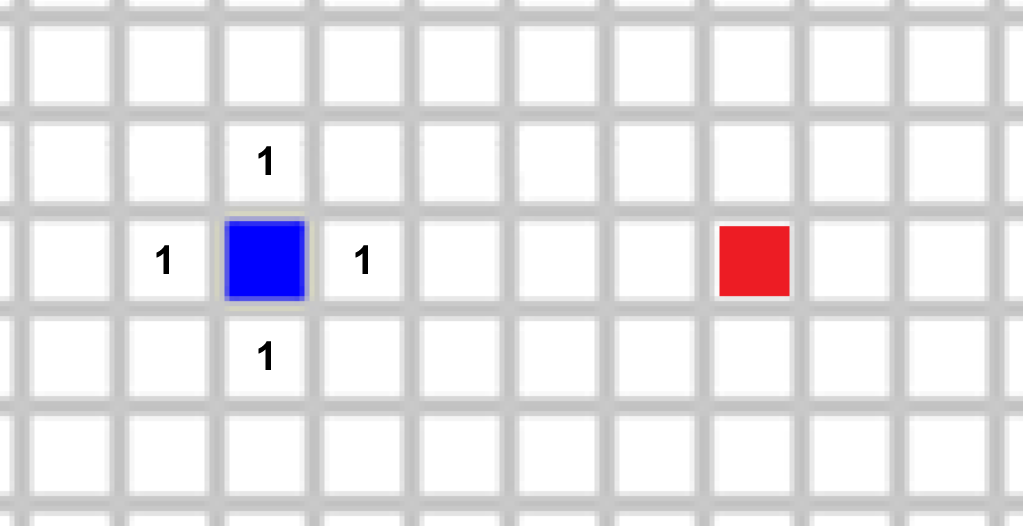
\includegraphics[scale=0.4]{imgs/dijkstra_step1.png}
\end{figure}
}

\frame{\frametitle{Dijkstra in action}
Step 2. Visit the closest vertex from the source. In this case we just picked the upper cell from the 4 closest vertices.
\begin{figure} 
\centering
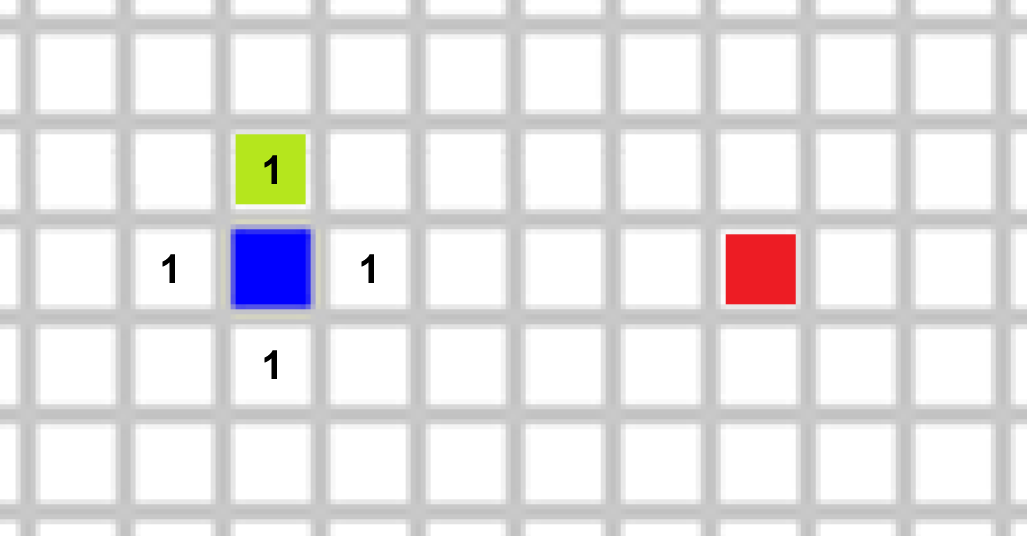
\includegraphics[scale=0.4]{imgs/dijkstra_step2.png}
\end{figure}
}

\frame{\frametitle{Dijkstra in action}
Step 3. Updates the distance to the vertices that are now reachable (but still unvisited) by the newly visited vertex. 
\begin{figure} 
\centering
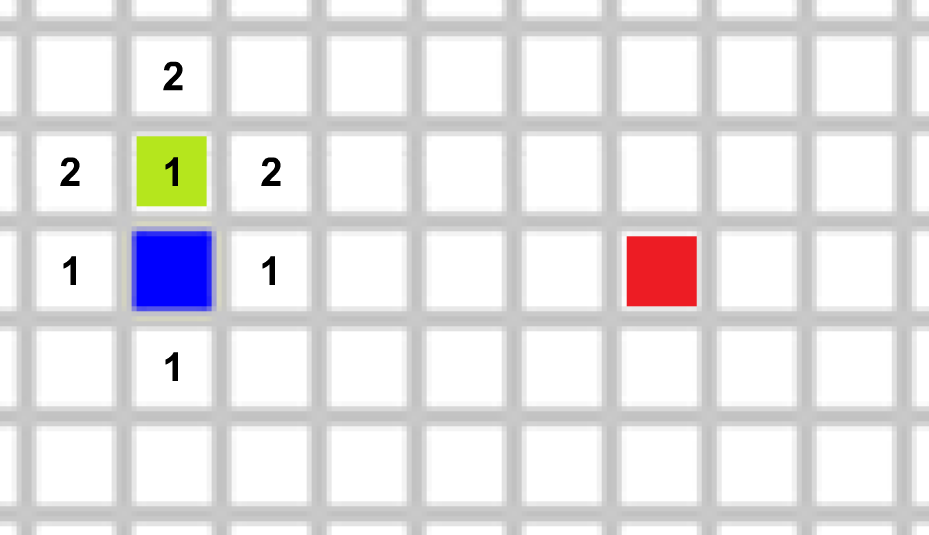
\includegraphics[scale=0.4]{imgs/dijkstra_step3.png}
\end{figure}
}

\frame{\frametitle{Dijkstra in action}
Step 4. Repeats the step 2-3 until it reached destination or all the vertex get marked visited.
\begin{figure} 
\centering
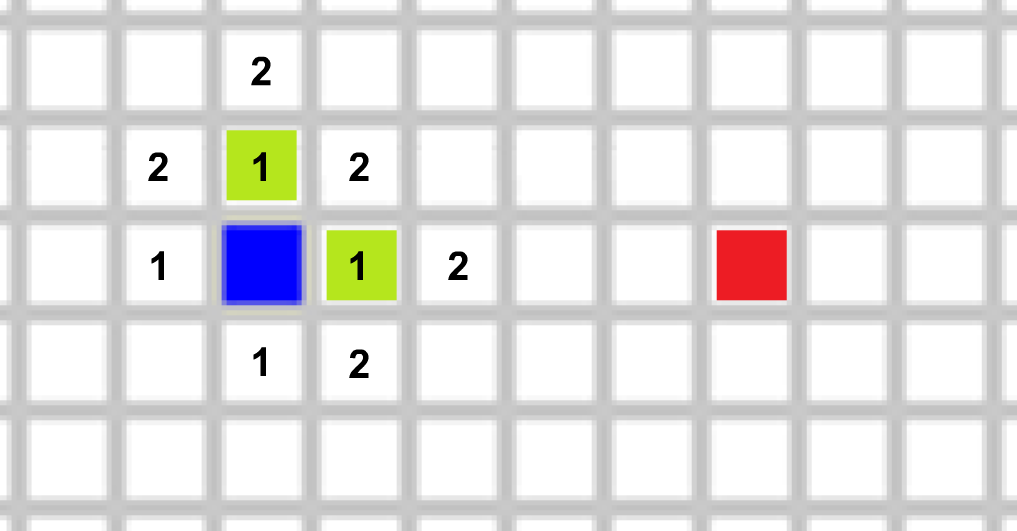
\includegraphics[scale=0.4]{imgs/dijkstra_step4.png}
\end{figure}
}

\frame{\frametitle{Dijkstra in action}
So when we are done, we might get something like this:
\begin{figure} 
\centering
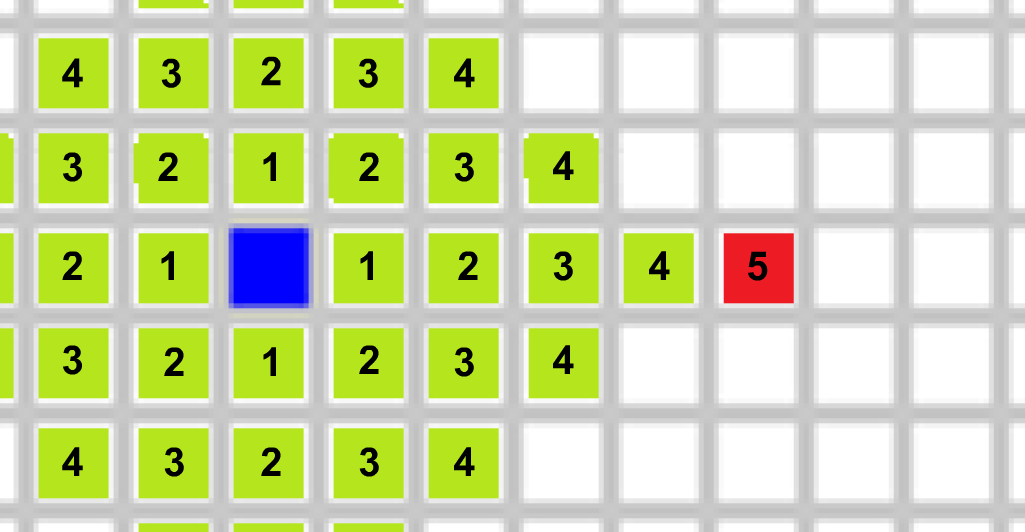
\includegraphics[scale=0.4]{imgs/dijkstra_done.png}
\end{figure}
}

\frame{\frametitle{Shortcoming of Dijkstra}
Dijkstra will find the shortest path eventually (proof can be seen at our research paper). However, we can see some shortcomings:
\begin{itemize}
  \item We were evaluating path that were "obviously" not part of the shortest path.
  \item Why find shortest path to all vertices when we only need to find one to $D$?
\end{itemize}
}

\subsection{A*}
\frame{\frametitle{A*}
\begin{itemize}
  \item "Dijkstra with a twist" \cite{Buckland}
  \item Dijkstra algorithm blindly selects vertex with minimum distance from $S$ each step. Instead, make a clever guess in each step where the algorithm selects a vertex that is likely part of the shortest path from $S$ to $D$.\cite{Buckland, HNR}
\end{itemize}
}
\frame{\frametitle{A*: Clever guess?}
For A* to work correctly and efficiently, the A* algorithm must guess each step that
\begin{itemize}
    \item Heuristic: \\
    Minimize unnecessary computation on finding sub-paths that are obviously not part of the optimal path\cite{HNR}, but also 
    \item Admissiblity: \\
    Should not ignore the sub-path that can be part of the optimal path\cite{HNR}.  
\end{itemize}
}

\frame{\frametitle{A* Algorithm}
The algorithm is almost the same as Dijkstra. Only difference is the step 2:

\begin{enumerate}
    \item ...
    \item Among the univisited vertices, visit the vertex that have the \textbf{lowest cost $f$} to the source vertex. 
    \item ...
    \item ...
\end{enumerate}
}

\frame{\frametitle{Cost?}
We define the cost of the vertex as a following:
\[ f(v) = g(v) + h(v) \]
\begin{itemize}
  \item $f(v) = $ total cost of the vertex $v$.
  \item $g(v) = $ exact distance from source to vertex $v$.
  \item $h(v) = $ estimated distance from vertex $v$ to destination. We will use euclidian distance between $v$ and $D$ as our estimation.
\end{itemize}
}

\frame{\frametitle{A* in action}
Let's revisit the step 2 of Dijkstra.
\begin{figure} 
\centering
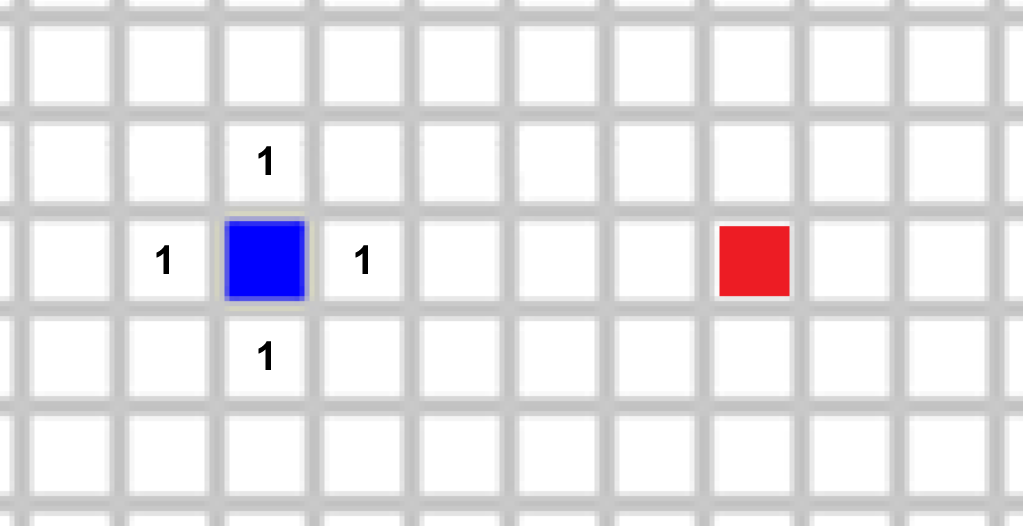
\includegraphics[scale=0.4]{imgs/dijkstra_step1.png}
\end{figure}
}

\frame{\frametitle{A* in action}
Instead of looking for the vertex that are closest to the source, look for the lowest cost $f$ as shown below.
\begin{figure} 
\centering
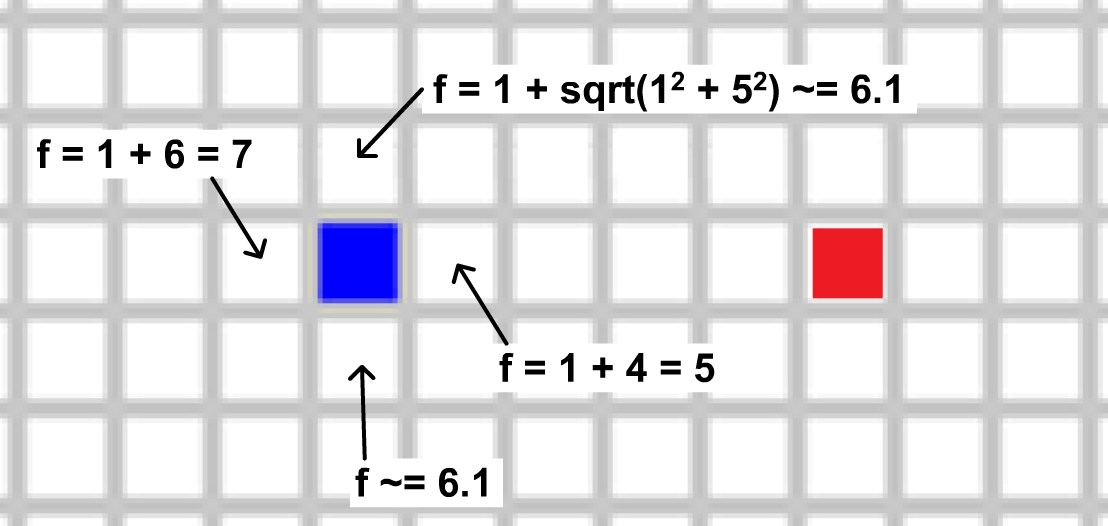
\includegraphics[scale=0.4]{imgs/astar_step1.PNG}
\end{figure}
}

\frame{\frametitle{A* in action}
Clearly, the winner is the right hand side vertex. \begin{figure} 
\centering
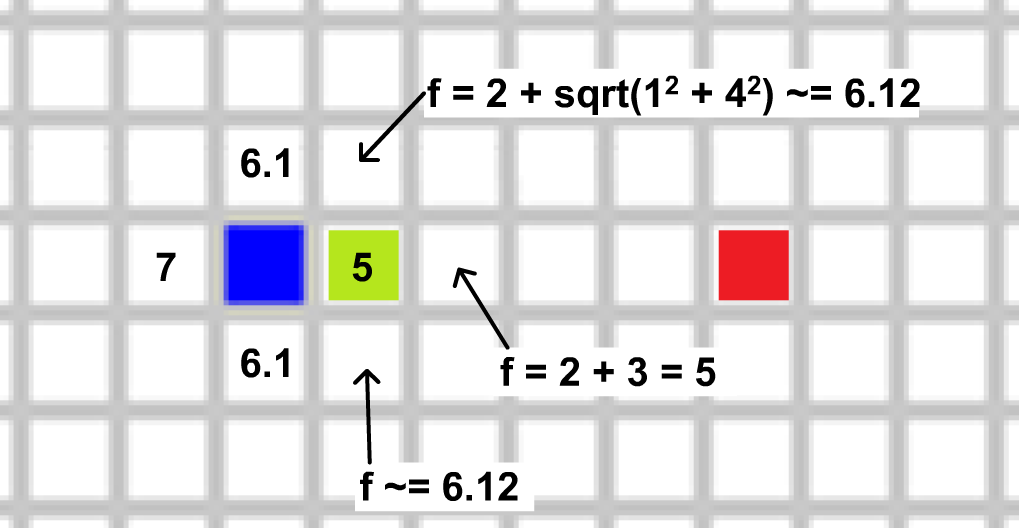
\includegraphics[scale=0.4]{imgs/astar_step2.PNG}
\end{figure}
}

\frame{\frametitle{A* in action}
This is similar to how human think, where we would unlikely consider traveling to a vertex in the opposite direction of a destination even if it is located close to the source. Rather, we would consider a nearby vertex closer to the destination unless it is deadend. 
}

\frame{\frametitle{Dijkstra in action}
So when we are done, we might get something like this:
\begin{figure} 
\centering
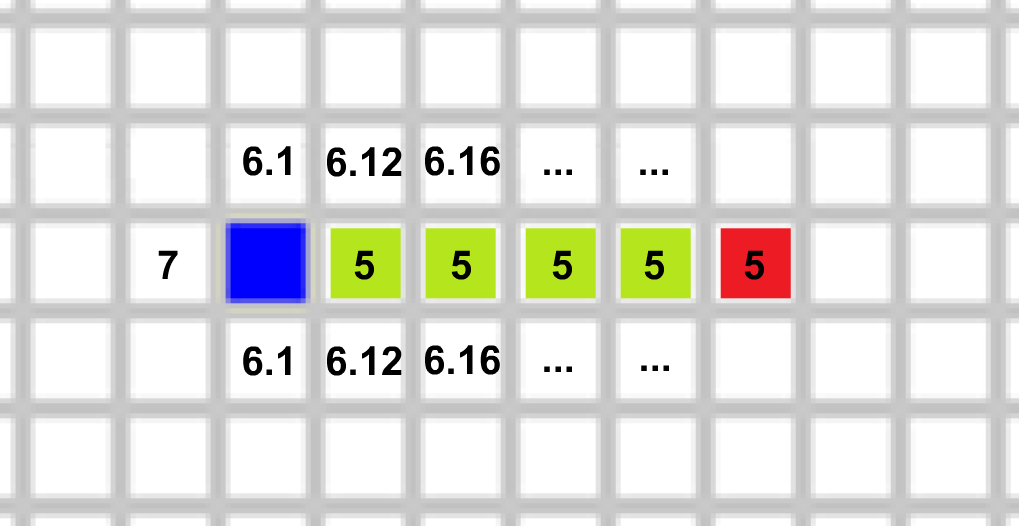
\includegraphics[scale=0.4]{imgs/astar_done.png}
\end{figure}
}
 

\frame{\frametitle{Shortcomings of A*}
In practice, a naive A* algorithm is still not sufficient for many modern applications with large network. 
\begin{enumerate}
  \item Many modern applications require computation to happen in real-time for hundreds, if not thousands, users/agents simultaneously\cite{Botea2004NearOH}.
  \item The shift to mobile applications has put more limitations on memory and CPU usage\cite{Botea2004NearOH}.
\end{enumerate}
}

\section{Hierarchical Path Finding}
\subsection{Using hierarchy to reduce complexity}
\frame{\frametitle{Hierarchical Path Finding}
So instead of running a shortest path algorithm on a large network, we run the shortest path algorithm inside the regional, more coarse grain, network. 
}
\frame{\frametitle{Using hierarchy to reduce compleixty}
The idea of Hierarchical Path Finding is to create a regional graph, then running a shortest path algorithm between the regions. 

\begin{figure} 
\centering
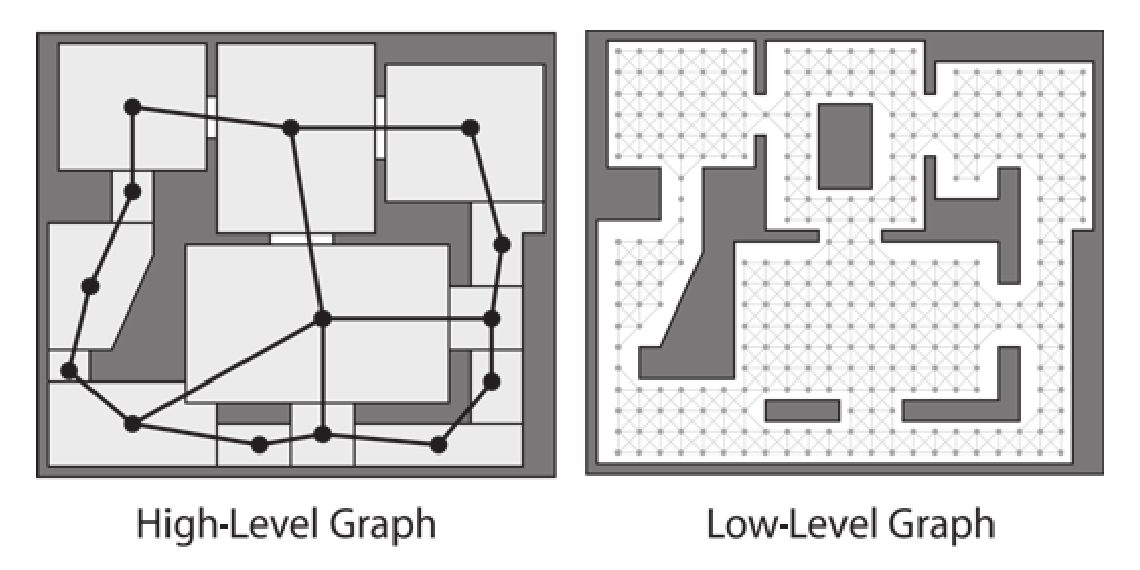
\includegraphics[scale=0.3]{imgs/hierarchy.png}
\caption{Forming regions (high-level graph) by clustering neighboring vertices. The figure was taken from \textit{Programming Game AI by Example} by Buckland\cite{Buckland}.} 
\end{figure}
}

\frame{\frametitle{How human use Hierarchial Path Finding in real life}
\begin{enumerate}
    \item Plan a route from Virginia Tech to a major highway entrance in Blacksburg.
    \item Plan a route from Blacksburg to Charlottesville.
    \item Plan a route from the highway exit in Charlottesville to the University of Virginia.
\end{enumerate}
}

\frame{\frametitle{Hierarchical Path Finding algorithm}
We apply the similar idea for our grid graph
\begin{enumerate}
  \item Run A* from source to the source regional entrance, 
  \item Run A* on regional level, from the source region to destination region, and 
  \item Run A* from destination region exit to destination.
\end{enumerate}
}

\subsection{Challenges}
\frame{\frametitle{Challenges}
Compare to Dijkstra and naive A*, there are more tunable variables that implementers need to consider
\begin{itemize}
  \item The number of hierarchy levels, 
  \item Cluster/region size, and 
  \item Placement of regional entrances/exits. 
  \item In practice, optimizations like preprocessing/caching regional routes and path smoothing may be necessary.
\end{itemize}
}
\frame{\frametitle{Simplification}
To avoid overwhelming the algorithm with optimization details, our implementation assume the following simplifications: 
\begin{enumerate}
  \item An input graph is static and known in advance, 
  \item 2 level of the hierarchy, 
  \item Preselected regional entrances/exits in reachable locations, 
  \item No preprocessing/caching, and 
  \item No path refinement or smoothing.
\end{enumerate}
}

\frame{\frametitle{Regional entrances/exits}
\begin{figure} 
\centering
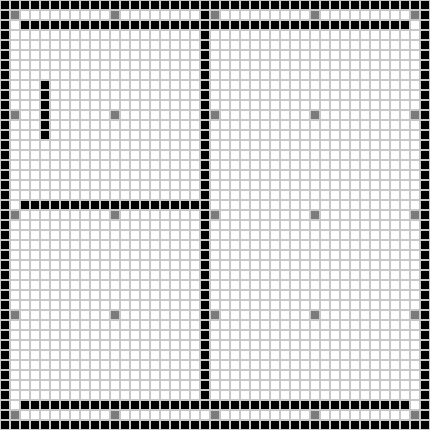
\includegraphics[scale=0.4]{imgs/regional_points.png}
\caption{Regional entrances/exits placement for experiment 1-3.} 
\end{figure}
}

\subsection{Experiment results}
\frame{\frametitle{Experiment setup 1}
\begin{figure} 
\centering
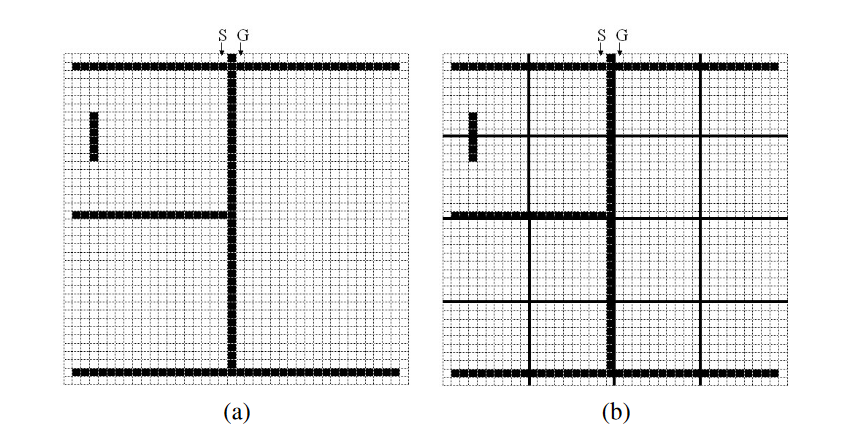
\includegraphics[scale=0.5]{imgs/experiment_setup.png}
\caption{(a) The 40 X 40 maze used in our example. The obstacles are painted in black. $S$ and $G$ are the start and the goal nodes. (b) The bold lines show the boundaries of the 10x 10 clusters\cite{Botea2004NearOH}.} 
\end{figure}
}
\frame{\frametitle{Experiment results 1}
\begin{center}
\begin{tabular}{| c | c | c | c | }
    \hline
     & Dijkstra & A* & Hierarchical Path Finding \\
    \hline
    \# of vertices visited & 1541 & 1523 & 993 \\
    \hline
    Path length & 159 & 159 & 176 \\
    \hline
    Time (ms) & 549.95 & 583.56 & 18.32 \\
    \hline
\end{tabular}

\end{center}
\begin{figure} 
\centering
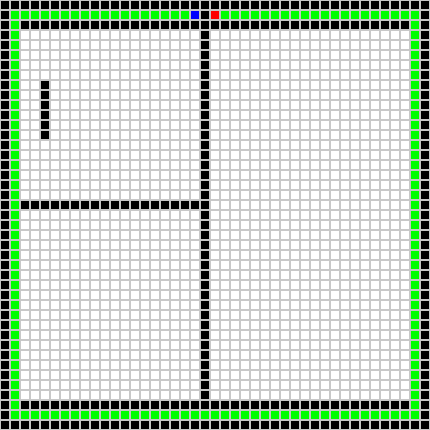
\includegraphics[scale=0.35]{imgs/exp_result1.png}
\end{figure}
}

\frame{\frametitle{Experiment setup 2}
\begin{figure} 
\centering
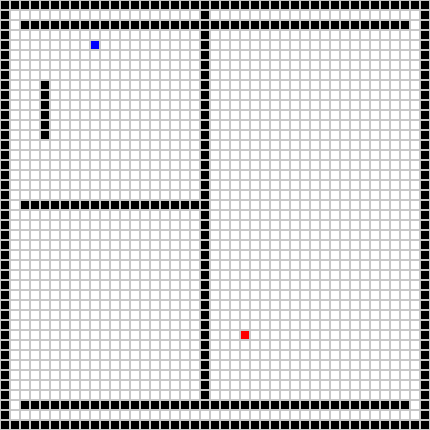
\includegraphics[scale=0.35]{imgs/exp2_setup.png}
\caption{Gird graph for experiment 2. Blue vertex is the source and red vertex is the destination.} 
\end{figure}
}
\frame{\frametitle{Experiment results 2}
\begin{center}
\begin{tabular}{| c | c | c | c | }
    \hline
     & Dijkstra & A* & Hierarchical Path Finding \\
    \hline
    \# of vertices visited & 1033 & 858 & 610 \\
    \hline
    Path length & 111 & 111 & 140 \\
    \hline
    Time (ms) & 231.84 & 164.27 & 10.76 \\
    \hline
\end{tabular}

\end{center}
\begin{figure} 
\centering
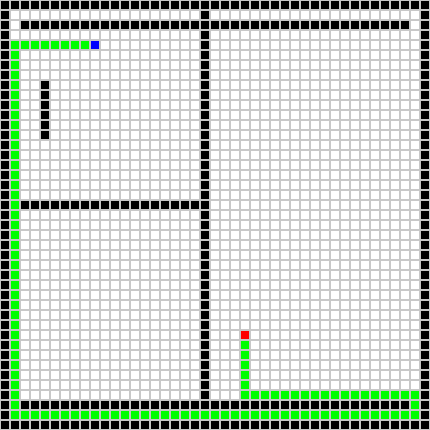
\includegraphics[scale=0.2]{imgs/exp2_dijkstra.png}
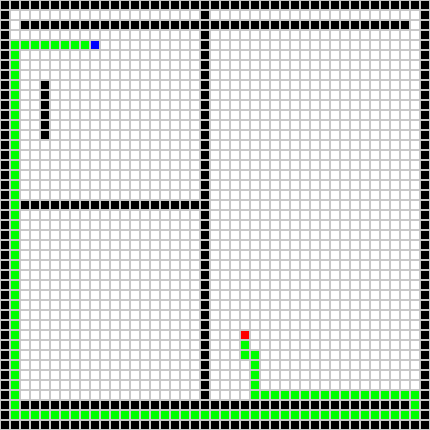
\includegraphics[scale=0.2]{imgs/exp2_astar.png}
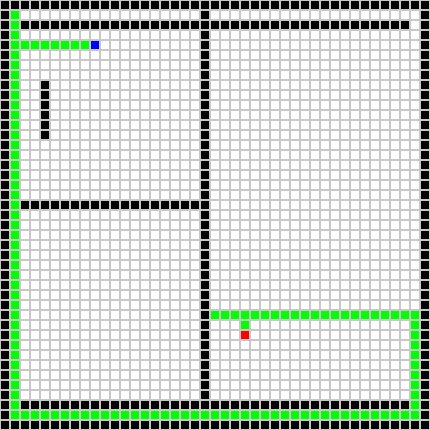
\includegraphics[scale=0.2]{imgs/exp2_hierarchical.png}
\caption{Results in a left to right order: Dijkstra, A*, Hierarchical Path Finding} 
\end{figure}
}

\frame{\frametitle{Experiment setup 3}
\begin{figure} 
\centering
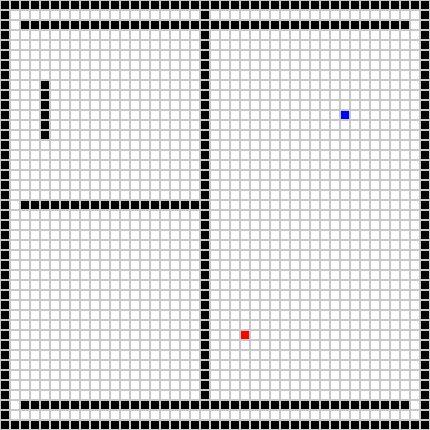
\includegraphics[scale=0.35]{imgs/exp3_setup.png}
\caption{Gird graph for experiment 3. Blue vertex is the source and red vertex is the destination.} 
\end{figure}
}
\frame{\frametitle{Experiment results 3}
\begin{center}
\begin{tabular}{| c | c | c | c | }
    \hline
     & Dijkstra & A* & Hierarchical Path Finding \\
    \hline
    \# of vertices visited & 740 & 329 & 285 \\
    \hline
    Path length & 33 & 33 & 44 \\
    \hline
    Time (ms) & 149.64 & 41.82 & 6.46 \\
    \hline
\end{tabular}

\end{center}
\begin{figure} 
\centering
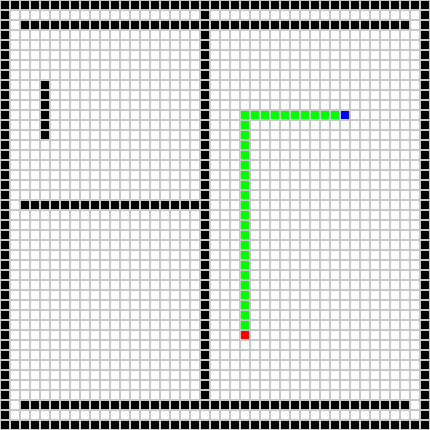
\includegraphics[scale=0.2]{imgs/exp3_dijkstra.png}
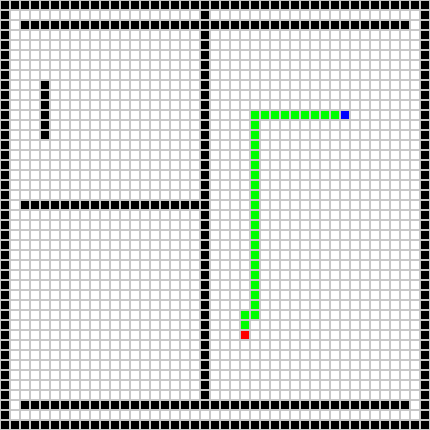
\includegraphics[scale=0.2]{imgs/exp3_astar.png}
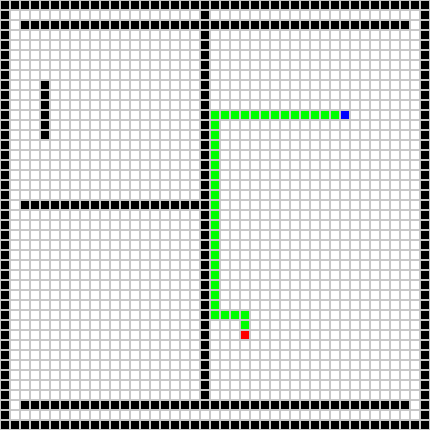
\includegraphics[scale=0.2]{imgs/exp3_hierarchical.png}
\caption{Results in a left to right order: Dijkstra, A*, Hierarchical Path Finding} 
\end{figure}
}


\section{Limitations}
\subsection{Near optimal path}
\frame{\frametitle{Limitations}
\begin{itemize}
  \item Hierarchical Path Finding does not guarantee the shortest path between the source and destination. 
  \item The \textit{Near Optimal Hierarchical Path-Finding} apply a path-smoothing procedure to make a path found by Hierarchical Path Finding within $1\%$ optimal compared to shortest path\cite{Botea2004NearOH}.
\end{itemize}
}

\frame{\frametitle{References}
\bibliographystyle{plain}
\bibliography{references.bib}
}

\end{document}